% Document: Bachelor Thesis: Minimal Problem Solver Generator
% Author: Pavel Trutman

\documentclass[msc]{cmpthesis}
\usepackage{indentfirst}
\usepackage{enumitem}

\startThesisInfo
\title{Minimal Problem Solver Generator}
\author{Pavel Trutman}
\CMPAdvisor{Ing. Tom\'a\v s Pajdla, PhD.}
\CMPReportNo{}
\CMPAcknowledgement{\centering Acknowledge grants here. Use centering
   if the text is too short.}

\CMPEmail{pavel.trutman@fel.cvut.cz}
\CMPDocumentURL{http://cmp.felk.cvut.cz/~trutmpav/theses/bsc-pavel-trutman.pdf}
\stopThesisInfo

% ============================== your definitions (abbreviations etc.)
%\def\Ax{\mathbf{A}_x}
\setitemize{noitemsep,topsep=0.2cm,parsep=0.2cm,partopsep=0pt,leftmargin=1cm}

% =========================================================== settings
%\graphicspath{{fig-ch01/}{fig-ch02/}}
\graphicspath{{images/}}

% ========================================================== text body
\begin{document}

\maketitle[3]

\cleardoublepage\def\thepage{\roman{page}}\setcounter{page}{3}
\mbox{}\vfill

{\let\clearpage\relax\par \chapter*{Acknowledgements}}
I would like to thank my advisor Tom\'a\v s Pajdla for introducing me into Gr\"obner basis methods for solving polynomial systems and for his guidance and advices which enabled me to finish this thesis. I would also like to thank Zuzana K\'ukelov\'a for presenting me the automatic generator and for her comments to improvements I have implemented. Special thanks go to my family for all their support.

\clearpage
\chapter*{Abstract}\chapter*{Abstract}
Many problems in computer vision lead to polynomial systems solving. Therefore, we need an easy way how to generate an efficient solver for each problem. On this purpose, the automatic generator has been presented. In this thesis, we improve the automatic generator so we will be able to generate more efficient and numerically stable solvers.

To improve the automatic generator we review and implement several methods used in the state of the art Gr\"obner basis solvers. Especially, we focus on the $F_4$ Algorithm by Jean-Charles Faug\`ere. Solvers, generated by the automatic generator, can be sped up when efficient methods are used to work with sparse matrices. We describe and implement method which is based on matrix partitioning. This method significantly speeds up the Gauss-Jordan elimination of sparse matrices.

We demonstrate the enhancements of the automatic generator on several important minimal problems. We show that the solvers generated by the new automatic generator are faster and numerically more stable than the solvers generated by the old version of the automatic generator.

\paragraph{Keywords:} computer vision, robotics, minimal problems, polynomials equations, Gr\"ob\-ner basis

\begin{otherlanguage}{czech}
\chapter*{Abstrakt}
Mnoho problémů v počítačovém vidění vede na řešení polynomiálních rovnic. Proto potřebujeme jednoduchý způsob, jak generovat efektivní postupy řešení každého z~prob\-lémů. Z tohoto důvodu byl představen automatický generátor. V této práci vylepšíme automatický generátor, takže budeme schopni generovat ještě rychlejší a numericky stabilnější postupy řešení polynomiálních systémů.

Abychom mohli vylepšit automatický generátor, prozkoumáme a následně implementujeme několik metod používaných v současných nástrojích na řešení soustav polynomiálních rovnic pomocí Gr\"obnerových bází. Zaměříme se zejména na algoritmus $F_4$ představený Jean-Charlesem Faug\`erem. Postupy řešení problémů, vygenerované pomocí automatického generátoru, mohou být ještě dále zrychleny, pokud použijeme efektivní metody pro práci s řídkými maticemi. Popíšeme a implementujeme metodu, která je založená na rozkladu matic. Tato metoda výrazně urychluje Gauss-Jordanovu eliminaci řídkých matic.

Vylepšení automatického generátoru předvedeme na několika významných mini\-mál\-ních problémech. Ukážeme, že postupy řešení problémů vygenerované novým automatickým generátorem jsou rychlejší a numericky stabilnější než postupy vygenerované původní verzí automatického generátoru.

\paragraph{Klíčová slova:} počítačové vidění, robotika, minimální problémy, polynomiální rovnice, Gr\"obnerovy báze
\end{otherlanguage}

\clearpage
\chapter*{Resum\'e}Text of resum\'e\dots

\endinput

\cleardoublepage\def\thepage{\arabic{page}}\setcounter{page}{1}
\tableofcontents\pagestyle{headings}

\startAbbreviations[AHA! Some optional explanation before the
list. Indentation can be set by the command
{\ttfamily $\backslash$setlength\{$\backslash$AbbrvIndent\}\{5em\}}.]
\abbrv[1D]    one dimension(al)
\abbrv[2D, 3D, \dots]
              two dimension(al), three dimension(al), two dimension(al),
              three dimension(al), two dimension(al), three
              dimension(al), two dimension(al), three dimension(al), \dots
\abbrv[AAM]   active appearance model
\abbrv[AI]    artificial intelligence
\abbrv[ASM]   active shape model
\abbrv[B-rep] boundary representation
\abbrv[BBN]   Bayesian belief networks
\stopAbbreviations

\endinput


\chapter{Introduction}
Here comes introduction.


\chapter{Polynomial system solving}
Firstly we review the state of the art algorithms for computing Gr\"obner basis. Better understanding of these algorithms helps us to integrate them into polynomial solving algorithms based on Gr\"obner basis computation more efficiently.

\section{Buchberger Algorithm}
Buchberger Algorithm \cite{Buchberger65}, which was invented by Bruno Buchberger, was the first algorithm for computing Gr\"obner basis. The algorithm is described in details in \cite{Becker93, Cox-Little-Shea97}.

\subsection{First implementation}
The first and easy, but very inefficient implementation of the Buchberger Algorithm, Algorithm \ref{alg:simpleBuchberger}, is based on the observation that we can extend a set $F$ of polynomials to a Gr\"obner basis only by adding all non-zero remainders $\overline{S(f_i, f_j)}^F$ of all pairs from $F$ into $F$ until there is no non-zero remainder generated.

The main disadvantage of this simple algorithm is that so constructed Gr\"obner basis are often bigger than necessary. This implementation of the algorithm is also very inefficient because many of the S-polynomials that are constructed from the critical pairs are reduced to zero so after spending effort on computing them, there is nothing to add to the Gr\"obner basis $G$. How to decide which pairs need not be generated is described next.

\begin{algorithm}[ht]
  \begin{algorithmic}[1]
    \Require
      \Statex $F$ a finite set of polynomials
    \Ensure
      \Statex $G$ a finite set of polynomials
      \Statex

    \State $G \gets F$
    \State $B \gets \left\{\left\{g_1, g_2\right\}\ |\ g_1, g_2 \in G,\ g_1 \neq g_2\right\}$
    \While{$B \neq \emptyset$}
      \State select $\left\{g_1, g_2\right\}$ from $B$
      \State $B \gets B\backslash\left\{\left\{g_1, g_2\right\}\right\}$
      \State $h \gets S(g_1, g_2)$
      \State $h_0 \gets \overline{h}^G$
      \If{$h_0 \neq 0$}
        \State $B \gets B \cup \left\{\left\{g, h_0\right\}\ |\ g\in G\right\}$
        \State $G \gets G \cup \left\{h_0\right\}$
      \EndIf
    \EndWhile

    \State \Return $G$

  \end{algorithmic}
  \caption{Simple Buchberger Algorithm}
  \label{alg:simpleBuchberger}
\end{algorithm}



\subsection{Improved Buchberger Algorithm}
\label{subsec:ImprovedBuchberger}
The combinatorial complexity of the simple implementation of the Buchberger Algorithm can be reduced by testing out certain S-polynomials which need not be considered. To know which pairs can be deleted without treatment, we use the first and the second Buchberger's criterion \cite{Becker93}. Sometimes, we can even delete certain polynomials from the set $G$ completely, knowing that every critical pair they will generate will reduce to zero and hence these polynomials themselves will be superfluous in the output set. In the next few paragraphs we will describe the implementation of the Improved Buchberger Algorithm and of the function \textit{Update}, which deletes superfluous polynomials from $G$, according to Gebauer and M\"oller \cite{Gebauer-Moller88}.

The Improved Buchberger Algorithm, Algorithm \ref{alg:improvedBuchberger}, has the same structure as the Simple Algorithm. The function \textit{Update} is used at the beginning of the Improved Buchberger Algorithm to initialize the set $B$ of critical pairs and the Gr\"obner basis $G$ from the input set $F$ of polynomials and at every moment when a new non-zero polynomial $h_0 = \overline{h}^G$ of an S-polynomial $h$ has been found and the sets $B$ and $G$ are about to be updated.

\begin{algorithm}[ht]
  \begin{algorithmic}[1]
    \Require
      \Statex $F$ a finite set of polynomials
    \Ensure
      \Statex $G$ a finite set of polynomials
      \Statex

    \State $G \gets \emptyset$
    \State $B \gets \emptyset$
    \While{$F \neq \emptyset$}
      \State select $f$ from $F$
      \State $F \gets F\backslash\{f\}$
      \State $(G, B) \gets Update(G, B, f)$
    \EndWhile
    \While{$B \neq \emptyset$}
      \State select $\{g_1, g_2\}$ from $B$
      \State $B \gets B\backslash \left\{\left\{g_1, g_2\right\}\right\}$
      \State $h \gets S(g_1, g_2)$
      \State $h_0 \gets \overline{h}^G$
      \If{$h_0 \neq 0$}
        \State $(G, B) \gets Update(G, B, h_0)$
      \EndIf
    \EndWhile

    \State \Return $G$

  \end{algorithmic}
  \caption{Improved Buchberger Algorithm}
\end{algorithm}


Now, let us look at the function \textit{Update}, Algorithm \ref{alg:update}. First, it makes pairs from the new polynomial $h$ and all polynomials from the set $G_{old}$ and puts them into the set $C$. The first while loop (lines \ref{alg:update:w1b} -- \ref{alg:update:w1e}) iterates over all pairs in the set $C$. In each iteration it select a pair $\{h, g_1\}$ from the set $C$ and removes it from the set. Then it looks for another pair $\{h, g_2\}$ from the set $C$ or the set $D$. If does not exists a pair $\{h, g_2\}$ such that $(h, g_2, g_1)$ is a Buchberger triple, then the pair $\{h, g_1\}$ is put into the set $D$. The triple $(h, g_2, g_1)$ of polynomials $h$, $g_1$ and $g_2$ is a Buchberger triple if the equivalent conditions 

\begin{eqnarray}
	\LM(g_2) &|& \lcm(\LM(h), \LM(g_1))\\
	\lcm(\LM(h), \LM(g_2) ) &|& \lcm(\LM(h), \LM(g_1))\\
	\lcm(\LM(g_2), \LM(g_1)) &|& \lcm(\LM(h), \LM(g_1))
\end{eqnarray}
are satisfied. From the second Buchberger's criterion, we know that if a Buchberger triple $(h, g_2, g_1)$ shows up in the Buchberger Algorithm and the pairs $\{g_1, g_2\}$ and $\{h, g_2\}$ are amongs the critical pairs, then the pair $\{h, g_1\}$ need not be generated. That means in the code that such a pair is not moved from the set $C$ to the set $D$ but it is only removed from the set $C$. This while loop keeps all pairs $\{h, g_1\}$ where LM$(h)$ and LM$(g_1)$ are disjoint, i.e. LM$(h)$ and LM$(g_1)$ have no variable in common. The reason of this is that if two or more pairs in $C$ have the same lcm of their leading monomials, then there is a choice which one should be deleted. So we keep the pair where the leading monomials are disjoint. Pairs with disjoint leading monomials are removed in the second while loop, so we eventually remove them all.

The second while loop (lines \ref{alg:update:w2b} -- \ref{alg:update:w2e}) eliminates all pairs with disjoint leading monomials. We can remove such pairs thanks to the first Buchberger's criterion. All remaining pairs are stored in the set $E$.

The third while loop (lines \ref{alg:update:w3b} -- \ref{alg:update:w3e}) eliminates pairs $\{g_1, g_2\}$ where $(g_1, h, g_2)$ is a Buchberger triple from the set $B_{old}$. Then the updated set of the old pairs and the new pairs are united into the set $B_{new}$.

Finally, the last while loop (lines \ref{alg:update:w4b} -- \ref{alg:update:w4e}) removes all polynomials $g$ whose leading monomial is a multiple of the leading monomial of $h$ from the set $G_{old}$. We can eliminate such polynomials for two reasons. Firstly, LM$(h) \mid$ LM$(g)$ implies LM$(h) \mid$ lcm(LM$(g)$, LM$(f)$) for arbitrary polynomial $f$. We can see that $(g, h, f)$ is a Buchberger triple for any $f$ which in future appears in the set $G$. Moreover, polynomial $g$ will not be missed at the end, because in the Gr\"obner basis $G$, polynomials with leading monomials which are multiples of leading monomials of another polynomial from $G$ are superfluous, i.e. they will be eliminated in the reduced Gr\"obner basis.

In the end of the function, the polynomial $h$ is added into the Gr\"obner basis $G_{new}$. The output of the function \textit{Update} is the Gr\"obner basis $G_{new}$ and the set $B_{new}$ of critical pairs.

\begin{algorithm}[htp]
  \begin{algorithmic}[1]
    \Require
      \Statex $G_{old}$ a finite set of polynomials
      \Statex $B_{old}$ a finite set of pairs of polynomials
      \Statex $h$ a polynomial such that $h \neq 0$
    \Ensure
      \Statex $G_{new}$ a finite set of polynomials
      \Statex $B_{new}$ a finite set of pairs of polynomials
      \Statex

    \State $C \gets \left\{\left\{h, g\right\}\ |\ g\in G_{old}\right\}$
    \State $D \gets \emptyset$
    \While{$C\neq \emptyset$}
      \State select $\{h,g_1\}$ from $C$
      \State $C \gets C\backslash \{\{h, g_1\}\}$
      \IfML{LM$(h)$ and LM$(g_1)$ are disjoint \textbf{or}}
        \StatexIndent[3](lcm(LM$(h)$, LM$(g_2)$) $\nmid$ lcm(LM$(h)$, LM$(g_1)$) for all $\{h, g_2\}\in C$ \textbf{and}
        \StatexIndent[3]lcm(LM$(h)$, LM$(g_2)$) $\nmid$ lcm(LM$(h)$, LM$(g_1)$) for all $\{h, g_2\} \in D$) \algorithmicthen
        \State $D \gets D \cup \{\{h, g_1\}\}$
      \EndIf
    \EndWhile

    \State $E \gets \emptyset$

    \While{$D \neq \emptyset$}
      \State select $\{h, g\}$ from $D$
      \State $D \gets D\backslash \{\{h, g\}\}$
      \If{LM$(h)$ and LM$(g)$ are not disjoint}
        \State $E \gets E \cup \{\{h, g\}\}$
      \EndIf
    \EndWhile

    \State $B_{new} \gets \emptyset$

    \While{$B_{old} \neq \emptyset$}
      \State select $\{g_1, g_2\}$ from $B_{old}$
      \State $B_{old} \gets B_{old} \backslash \{\{g_1, g_2\}\}$
      \IfML{LM$(h) \nmid$ lcm(LM$(g_1)$, LM$(g_2)$) \textbf{or}}
        \StatexIndent[3]lcm(LM$(g_1)$, LM$(h)) = $ lcm(LM$(g_1)$, LM$(g_2)$) \textbf{or}
        \StatexIndent[3]lcm(LM$(h)$, LM$(g_2)) = $ lcm(LM$(g_1)$, LM$(g_2)$) \algorithmicthen
        \State $B_{new} \gets B_{new} \cup \{\{g_1, g_2\}\}$
      \EndIf
    \EndWhile

    \State $B_{new} \gets B_{new} \cup E$
    \State $G_{new} \gets \emptyset$
    
    \While{$G_{old} \neq \emptyset$}
      \State select $g$ from $G_{old}$
      \State $G_{old} \gets G_{old} \backslash \{g\}$
      \If{LM$(h)$ $\nmid$ LM$(g)$}
        \State $G_{new} \gets G_{new} \cup \{g\}$
      \EndIf
    \EndWhile

    \State \Return $(G_{new}, B_{new})$

  \end{algorithmic}
  \caption{Update}
\end{algorithm}


\section{$F_4$ Algorithm}
The $F_4$ Algorithm \cite{F4} by Jean-Charles Faug\`ere is an improved version of the Buchberger's Algorithm. The $F_4$ replaces the classical polynomial reduction found in the Buchberger's Algorithm by a simultaneous reduction of several polynomials. This reduction mechanism is achieved by a symbolic precomputation followed by Gaussian elimination implemented using sparse linear algebra methods. $F_4$ speeds up the reduction step by exchanging multiple polynomial divisions for row-reduction of a single matrix.

\subsection{Improved Algorithm $F_4$}
The main function of the $F_4$ Algorithm, Algorithm \ref{alg:F4}, consists of two parts. The goal of the first part is to initialize the whole algorithm.

First, it generates the set $P$ of critical pairs and initializes the Gr\"obner basis $G$. This is done by taking each polynomial from the input set $F$ and calling the function \textit{Update} on it, which updates the set $P$ of pairs and the set $G$ of basic polynomials.

The second part of the algorithm generates new polynomials and adds them into the set $G$. In each iteration, it selects some pairs from $P$ using the function \textit{Sel}. Many selection strategies are possible and is still an open question how to best select the pairs. Some selection strategies are described in the section \ref{subsec:F4:sel} on page \pageref{subsec:F4:sel}. Then, it splits each selected pair $\{f_1, f_2\}$ into two tuples. The first tuple contains the first polynomial $f_1$ of the pair and the monomial $m_1$ such that $\textrm{LM}(m_1 \times f_1) = \textrm{lcm}(\textrm{LM}(f_1),\textrm{LM}(f_2))$. The second tuple is constructed in the same way from the second polynomial $f_2$ of the pair. All tuples from all selected pairs are put into the set $L$, i.e. duplicates are removed.

Next, function \textit{Reduction} is called on the set $L$. It stores result in the set $\tilde{F}^+$. In the end of the algorithm it iterates through all new polynomials in the set $\tilde{F}^+$ and calls the function \textit{Update} on each of them. This generates new pairs into the set $P$ of critical pairs and extends the Gr\"obner basis $G$.

This algorithm terminates when the set $P$ of pairs is empty. Then the set $G$ is a Gr\"obner basis and it is the output of the algorithm.

\begin{algorithm}[ht]
  \begin{algorithmic}[1]
    \Require
      \Statex $F$ a finite set of polynomials
      \Statex $Sel$ a function $List(Pairs) \to List(Pairs)$ such that $Sel(l) \neq \emptyset$ if $l\neq\emptyset$
    \Ensure
      \Statex $G$ a finite set of polynomials
      \Statex

    \State $G \gets \emptyset$
    \State $P \gets \emptyset$
    \State $d \gets 0$

    \While{$F \neq \emptyset$}
      \State select $f$ form $F$
      \State $F \gets F\backslash \{f\}$
      \State $(G, P) \gets Update(G, P, f)$
    \EndWhile
    
    \While{$P\neq\emptyset$}
      \State $d \gets d + 1$
      \State $P_d \gets Sel(P)$
      \State $P \gets P\backslash P_d$
      \State $L_d \gets Left(P_d) \cup Right(P_d)$
      \State $(\tilde{F}^+_d, F_d) \gets Reduction(L_d, G, (F_i)_{i=1,\ldots,(d-1)})$
      \For{$h\in\tilde{F}^+_d$}
        \State $(G, P) \gets Update(G, P, h)$
      \EndFor
    \EndWhile
    \State \Return $G$

  \end{algorithmic}
  \caption{Improved Algorithm $F_4$}
  \label{alg:F4}
\end{algorithm}



\subsection{Function Update}
In the $F_4$ Algorithm the standard implementation of the Buchberger's Criteria such as the Gebauer and M\"oller installation \cite{Gebauer-Moller88} is used. Details about the function \textit{Update} can be found in the section \ref{subsec:ImprovedBuchberger}. The pseudocode of the function is shown in Algorithm \ref{alg:update}.

\subsection{Function Reduction}
Function \textit{Reduction}, Algorithm \ref{alg:reduction}, performs polynomial division using methods of linear algebra.

Input of the function \textit{Reduction} is a set $L$ containing tuples of monomial and polynomial. These tuples were constructed in the main function of the $F_4$ Algorithm from all selected pairs.

First, the function \textit{Reduction} calls the function \textit{Symbolic Preprocessing} on the set $L$. This returns a set $F$ of polynomials to be reduced. To use linear algebra methods to perform polynomial division, the polynomials have to be represented by a matrix. Each column of the matrix corresponds to a monomial. Columns have to be ordered with respect to the monomial ordering used so that the most right column corresponds to ``1''. Each row of the matrix corresponds to a polynomial from the set $F$. The matrix is constructed as follows. On the $(i, j)$ position in the matrix, we put the coefficient of the term corresponding to $j$-th monomial from the $i$-th polynomial from the set $F$.

We next reduce the matrix to a row echelon form using, for example, Gauss-Jordan elimination. Note that this matrix is typically sparse so we can use sparse linear algebra methods to save computation time and memory. After elimination, we construct resulting polynomials by multiplying the reduced matrix by a vector of monomials from the right.

In the end, the function returns the set $\tilde{F}^+$ of reduced polynomials such that their leading monomials are not leading monomials of any polynomial from the set $F$ of polynomials before reduction.

\begin{algorithm}[ht]
  \begin{algorithmic}[1]
    \Require
      \Statex $L$ a finite set of tuples of monomial and polynomial
      \Statex $G$ a finite set of polynomials
      \Statex $\mathcal{F} = (F_i)_{i=1,\ldots,(d-1)}$, where $F_i$ is finite set of polynomials
    \Ensure
      \Statex $\tilde{F}^+$ a finite set of polynomials
      \Statex $F$ a finite set of polynomials
      \Statex

    \State $F \gets Symbolic\ Preprocessing(L, G, \mathcal{F})$
    \State $\tilde{F} \gets$ Reduction to a Row Echelon Form of $F$
    \State $\tilde{F}^+ \gets \left\{f \in \tilde{F}\ |\ \textrm{LM}(f) \notin \textrm{LM}(F)\right\}$

    \State \Return $(\tilde{F}^+, F)$

  \end{algorithmic}
  \caption{Reduction}
\end{algorithm}



\subsection{Function Symbolic Preprocessing}
Function \textit{Symbolic Preprocessing}, Algorithm \ref{alg:symbolicPreprocessing}, starts with a set $L$ of tuples each containing a monomial and a polynomial. These tuples were constructed in the main function of the $F_4$ Algorithm from the selected pairs. Then, the tuples are simplified by the function \textit{Simplify} and after multiplying polynomials with corresponding monomials, the results are put into the set $F$.

Next, the function goes through all monomials in the set $F$ and for each monomial $m$ looks for some polynomial $f$ from the Gr\"obner basis $G$ such $m = m^\prime \times \textrm{LM}(f)$ where $m^\prime$ is some monomial. All such polynomials $f$ and monomials $m^\prime$ are after simplification multiplied and put into the set $F$. The goal of this search is to have for every monomial in $F$ a polynomial in $F$ with the same leading monomial. This will ensure that all polynomials from $F$ will be reduced for $G$ after polynomial division by linear algebra.

\begin{algorithm}[ht]
  \begin{algorithmic}[1]
    \Require
      \Statex $L$ a finite set of tuples of monomial and polynomial
      \Statex $G$ a finite set of polynomials
      \Statex $\mathcal{F} = (F_i)_{i=1,\ldots,(d-1)}$, where $F_i$ is finite set of polynomials
    \Ensure
      \Statex $F$ a finite set of polynomials
      \Statex

    \State $F \gets \big\{multiply($\textit{Simplify}$(m, f, \mathcal{F}))\ |\ (m, f)\in L\big\}$
    \State $Done \gets \textrm{LM}(F)$
    \While{$\textrm{M}(F) \neq Done$}
      \State $m$ an element of $\textrm{M}(F)\backslash Done$
      \State $Done \gets Done \cup \{m\}$
      \If{$m$ is top reducible modulo $G$}
        \State $m = m^\prime \cdot\textrm{LM}(f)$ for some $f \in G$ and some monomial $m^\prime$
        \State $F \gets F \cup \big\{multiply($\textit{Simplify}$(m^\prime, f, \mathcal{F}))\big\}$
      \EndIf
    \EndWhile

    \State \Return $F$

  \end{algorithmic}
  \caption{Symbolic Preprocessing}
  \label{alg:symbolicPreprocessing}
\end{algorithm}



\subsection{Function Simplify}
The function \textit{Simplify}, Algorithm \ref{alg:simplify}, simplifies a polynomial $m \times f$ which is a product of a given monomial $m$ and a polynomial $f$.

The function recursively looks for a monomial $m^\prime$ and a polynomial $f^\prime$ such that $\textrm{LM}(m^\prime\times f^\prime) = \textrm{LM}(m\times f)$. The polynomial $f^\prime$ is selected from all polynomials that have been reduced in previous iterations (sets $\tilde{F}$). We select polynomial $f^\prime$ such that the total degree of $m^\prime$ is minimal.

This is done in the function \textit{Symbolic Preprocessing} to insert polynomials that are mostly reduced and have a small number of monomials into the set $F$ of polynomials to be reduced. This of course speeds up following reduction.

\begin{algorithm}[ht]
  \begin{algorithmic}[1]
    \Require
      \Statex $m$ a monomial
      \Statex $f$ a polynomial
      \Statex $\mathcal{F} = (F_i)_{i=1,\ldots,(d-1)}$, where $F_i$ is finite set of polynomials
    \Ensure
      \Statex $(m^\prime, f^\prime)$ a non evaluated product of a monomial and a polynomial
      \Statex

    \For{$u \in$ list of all divisors of $m$}
      \If{$\exists j\ (1 \leq j \le d)$ such that $(u\times f) \in F_j$}
        \State $\tilde{F}_j$ is the Row Echelon Form of $F_j$
        \State there exists a (unique) $p\in \tilde{F}^+_j$ such that $\textrm{LM}(p) = \textrm{LM}(u\times f)$
        \If{$u\neq m$}
          \State \Return $Simplify(\frac{m}{u}, p, \mathcal{F})$
        \Else
          \State \Return $(1, p)$
        \EndIf
      \EndIf
    \EndFor

    \State \Return $(m, f)$

  \end{algorithmic}
  \caption{Simplify}
\end{algorithm}



\subsection{Selection strategy}
\label{subsec:F4:sel}
For the speed of the $F_4$ Algorithm, it is very important how the critical pairs from the list of all critical pairs $P$ are selected in each iteration. This of course depends on the implementation of the function \textit{Sel}. There are more possible selection strategies:

\begin{itemize}
  \item The easiest implementation is to select all pairs from $P$. In this case we reduce all critical pairs at the same time.
  \item If the function \textit{Sel} selects only one critical pair then the $F_4$ Algorithm is the Buchberger's Algorithm. In this case the \textit{Sel} function corresponds to the selection strategy in the Buchberger's Algorithm.
  \item The best function that Faug\`ere has tested is to select all critical pairs with a minimal total degree. Faug\`ere calls this strategy the \textit{normal strategy for} $F_4$. Pseudocode of this function can be found as Algorithm \ref{alg:sel}.
\end{itemize}

\begin{algorithm}[ht]
  \begin{algorithmic}[1]
    \Require
      \Statex $P$ a list of critical pairs
    \Ensure
      \Statex $P_d$ a list of critical pairs
      \Statex

    \State $d \gets min\left\{\textrm{deg}(\textrm{lcm}(p))\ |\ p\in P\right\}$
    \State $P_d \gets \left\{p\in P\ |\ \textrm{deg}(\textrm{lcm}(p)) = d\right\}$
    \State \Return $P_d$
  \end{algorithmic}
  \caption{Sel -- The normal strategy for $F_4$}
\end{algorithm}



\section{$F_5$ Algorithm}
The $F_5$ Algorithm \cite{F5} by Jean-Charles Faug\`ere.


\chapter{Automatic generator}
The automatic generator of Gr\"obner basis solvers is used to easily solve problems leading to systems of polynomial equations. These systems usually arise when solving minimal problems \cite{MinimalProblems} in computer vision. Typically, these systems are not trivial so special solvers have to be designed for concrete problems to achieve efficient and numerically stable solvers. But solvers generated for concrete problems can not be easily applied for similar or new problems and therefore the automatic generator was proposed in \cite{AutoGen}. Solvers generated by the automatic generator can be easily used to solve complex problems even by non-experts users.

The input of the automatic generator is a system of polynomial equations with a finite number of solutions and the output is a MATLAB or a Maple code that computes solutions of the given system for arbitary coefficients. One of the goals of this thesis is to improve previous implementation \cite{AutoGen} of the automatic generator to construct more efficient and numerically stable solvers.

The newest version of the automatic genenerator implemented in MATLAB can be downloaded from \cite{AutomaticGenerator}.

\section{Description of the automatic generator}
In this section we would like to briefly describe the procedure for generating solvers. The automatic generator consists of several independent modules, see Figure \ref{autogen:blockDiagram}. Since all these modules are independent, they can be easily improved or replaced by more efficient implementations. Next we describe each of these modules, full description can be found in \cite{AutoGen, KukelovaAlgMethods}.

\begin{figure}[ht]
  \centering
  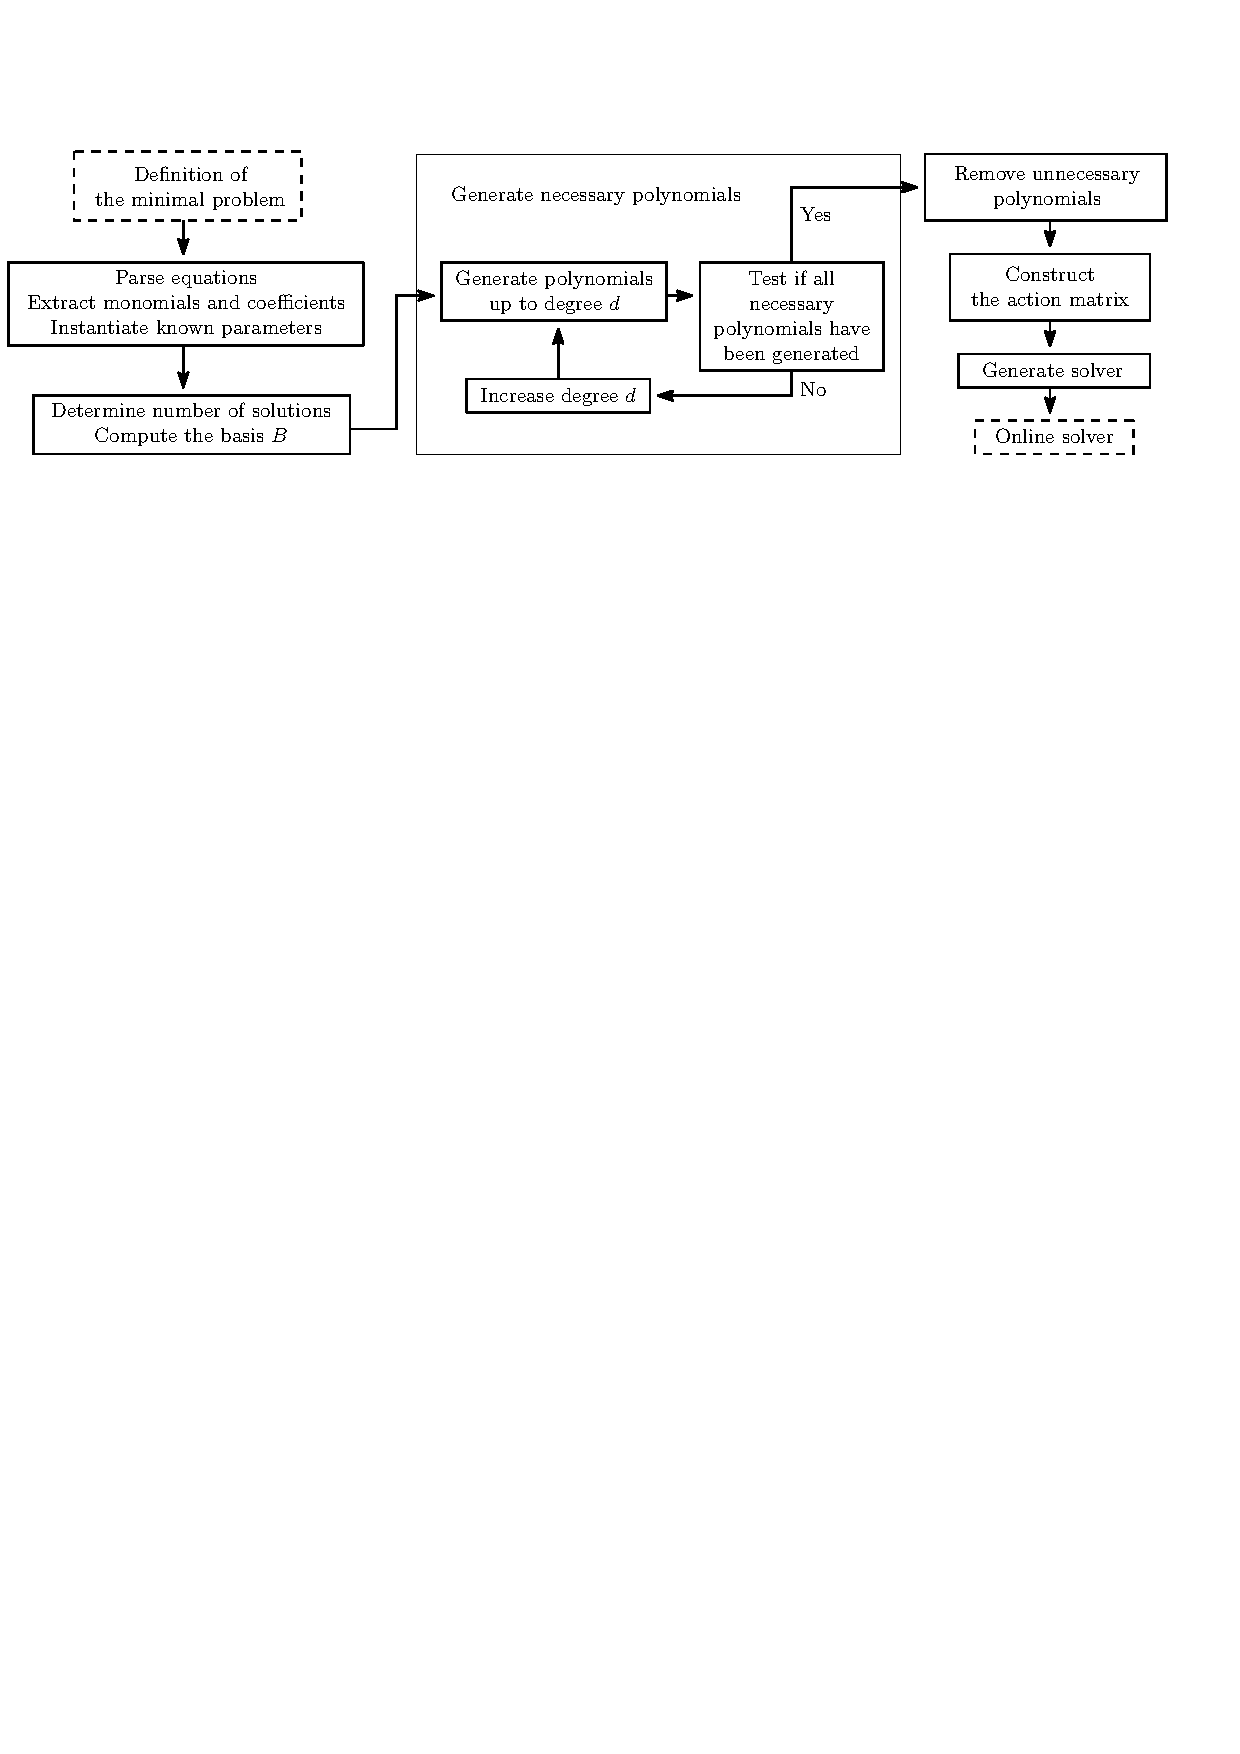
\includegraphics[width=0.95\textwidth]{AutomaticGenerator.pdf}
  \caption{Block diagram of the automatic generator}
  \label{autogen:blockDiagram}
\end{figure}

\subsection{Definition of the minimal problem}
Definitions of minimal problems are written in separate functions that are stored in the folder \texttt{minimalProblems}. Each of the definitions has to contain few necessary information about the minimal problem. First of all, the system of polynomial equations with symbolic variables and parameters has to be provided. Next we have to specify the list of unknown variables and known parameters. Optionally if we know the monomial basis $B$ of the polynomial system in advance we can specify it to save some computation time. The monomial basis $B$ is a set $\left\{m\ |\ \overline{m}^G = m\right\}$ where $m$ is a monomial and $G$ is the Gr\"obner basis of the given polynomial system. At last we have to set some settings for the automatic generator. We recommend to obtain the default settings by calling the function \textit{gbs\_InitConfig()} and only overwrite the settings we want to change. In the folder \texttt{minimalProblem} there are some examples which are self explanatory and can be used as templates to create new minimal problem definitions.

\subsection{Equations parser, Instantiating}
In the next step we have to parse the given equations, that means we extract used monomials and parameters and obtain total degrees of the polynomials. Then we instantiate each known parameter with a random number from $\mathbb{Z}_p$. We assign unique identifier to each used parameter. The reason is that we need to track the parameters through the process of adding polynomials in order to be able to restore the process in the solver generation module.

\subsection{Monomial basis $B$ computation}
We need to know the monomials basis $B$ to recognize when we have generated all polynomials that are necessary to build the action matrix. If the basis $B$ was not provided within the definition of the minimal problem we have to compute it by ourselves. Because in MATLAB there is no function or simple script to compute the basis we have to do it by calling an external software.

The most easy solution to implement is to use the Maple toolbox for MATLAB. This enables us to call Maple functions from the MATLAB environment directly. To use this option we have to set \texttt{cfg.GBSolver = @gbs\_findAlgB\_maple} in the settings of the automatic generator. Unfortunately it shows up that the symbolic toolbox provided by Maple in not compatible with the MATLAB symbolic toolbox in versions newer than R2008 so we do not recommend to use this option nowadays, but the option is still available to use on older computers.

The second implemented option is to use the algebraic geometry software Macaulay2 \cite{M2}. In the folder \texttt{gbsMacaulay} there is a template \texttt{code\_template.m2} into which we simply write the given polynomial system. This updated file is saved as \texttt{code.m2} which is executed by Macaulay2 and the results are parsed back in MATLAB. To set up this option we need to install the software Macaulay2 and set \texttt{cfg.GBSolver = @gbs\_findAlgB\_macaulay} in the automatic generator settings. A problem could be that the Macaulay2 is not easy to set up under the Windows OS. Therefore the installation file of Macaulay2 is provided within the automatic generator. The only thing that has to be done is to edit the file \texttt{calc.bat} in the folder \texttt{gbsMacaulay} and follow the instructions in the file.

Because of the modularity of the generator this part can be replaced by another function computing the monomial basis $B$.

The last option is to compute the basis $B$ in advance and set it into the definition of the minimal problem.

In the end we have check the number of solutions of the given polynomial system. If there is a finite number of solutions we can continue with the computation.

\subsection{Polynomial generator}
To be able to build the action matrix we have to generate enough polynomials such that after their reduction we get polynomials $q_i$ which have leading monomials from the set $\left(x_k \cdot B\right)\backslash B$ where $x_k$ is a variable and all remaining monomials are from the set $B$. That is the reason we had to compute the basis $B$ in the previous step.

In this part of the automatic generator we represent polynomials as row vectors so systems of polynomials can be represented by matrices. This representation enables us to easily multiplicate polynomials with monomials only by shifting the coefficients in the vectors or to reduce the whole polynomial systems by performing the Gauss-Jordan eliminations on the corresponding matrices.

Let $f_1, \dots, f_n$ are the polynomials from the input. Let $maxdeg$ is a maximal total degree of all polynomials $f_i$. At the beginning we put into the matrix $M$ all polynomials $\left\{m\times f_i\ |\ i = 1,\dots n;\ deg(m\times f_i) = deg(f_i),\dots, maxdeg\right\}$, where $m$ is a monomial. Now we perform the Gauss-Jordan elimination on the matrix $M$ and the result save as matrix $\tilde{M}$. Then we check if there exists a variable $x_k$ for which all required polynomials $q_i$ are present in $\tilde{M}$. If we find such a variable we can continue with the construction of the action matrix for the found variable. If not we have to add more polynomials to the matrix $M$. We increment $maxdeg$ by one and add all polynomials $\left\{m\times f_i\ |\ i = 1,\dots n;\ deg(m\times f_i) = maxdeg\right\}$ to the matrix $M$. Then we continue with the elimination and with the checking the action matrix requirements as written above. We repeat these steps until all required polynomials $q_i$ are generated so the action matrix can be built.

In this whole process we need to keep track how the matrix $M$ was built. Recall that each coefficient of the polynomials $f_i$ has unique identifier assigned in the equations parser. Because the whole matrix $M$ contains only the polynomials $f_i$ or their multiples with monomials therefore in the matrix $M$ appear only the coefficients from the polynomials $f_i$. We just have to keep the positions of the coefficients. This is done by matrix $M_c$. The matrix $M_c$ is built in the same time as the matrix $M$ by this way: if we put a coefficient into the matrix $M$ we also put the corresponding indentifier to the matrix $M_c$ at the same possition. The matrix $M_c$ enables us to recover the process of polynomials generation in the code generator module.

\subsection{Removing unnecessary polynomials and monomials}
Since in the previous step the polynomials were generated systematically there may appear some polynomials which are not necessary for the constructing of the action matrix. The goal of this part of the automatic generator is to remove as many as possible not necessary polynomials.

We can remove a polynomial $r$ from the matrix $M$ if the corresponding eliminated matrix $\tilde{M}$ still contains all required polynomials $q_i$. In this way we try to remove all polynomials from $M$.

Because the success of removing a polynomial depends on the previous removals, the number of removed polynomials depends on the ordering in which the polynomials are removed. In the automatic generator we start removing polynomials from the one with the largest leading monomial to the polynomial with the smallest leading monomial. Because it is very inefficient to remove polynomials one by one and perform each time an expensive Gauss-Jordan elimination, we can enhance the procedure by trying to remove more polynomials at the time. In the automatic generator there is used this heuristic: if we have successfully removed $k$ polynomials, we try to remove $2\cdot k$ polynomials in the next step. If the removal of $k$ polynomials have failed we try to remove $\frac{1}{4}k$ polynomials in the next step.

Moreover we can reduce the size of the matrix $M$ by removing unnecessary monomials. A monomial is unnecessary when its removal does not affect the building of the action matrix. We have to keep all monomials such that they are leading monomials of polynominals in the corresponding matrix $\tilde{M}$ and all monomials that are present in the basis $B$. All other monomials can be removed. If we remove all such unnecessary monomials then the matrix $M$ will have dimensions $n \times (n + N)$ where $n$ is the number of the polynomials in the matrix $M$ and $N$ is the number of solutions of the given system.

\subsection{Construction of the action matrix}
This part of the automatic generator starts with the eliminated matrix $\tilde{M}$ of polynomials and variable $x_k$ for which all required polynomials $q_i$ are present in the $\tilde{M}$.

Let us describe the construction of the action matrix in an informal and practical way rather than by using the theory. If the theory is needed it can be found in \cite{KukelovaAlgMethods}. The action matrix $M_{x_k}$ corresponding to the variable $x_k$ is a square matrix of dimensions $N \times N$ where $N$ is the number of elements of the monomial basis $B$. Each row and column corresponds to a monomial $b_i \in B$. Let the monomials $b_i$ are sorted such that if $b_l \prec b_k$ then $k < l$ where $\prec$ is a monomial ordering used. To the $i$-th row we put coefficients of the polynomial $m_i\ =\ \overline{(x_k \times b_i)}^F$ where $F$ are polynomials corresponding to $\tilde{M}$. Because $\tilde{M}$ is in a row echelon form there are two possibilities how the $i$-th row can be constructed:
\begin{enumerate}
  \item $x_k \times b_i\ =\ b_j$ for some $b_j \in B$\\
        That means that $x_k \times b_i$ is irreducible by $F$ and $m_i$ is a monomial in $B$. In this case we set $(i, j)\ =\ 1$ and $(i, k)\ =\ 0$ where $k\ \neq\ j$.
  \item $x_k \times b_i\ \neq\ b_j$ for all $b_j \in B$\\
	  In this case there is $f$ such that $\LM(m_i)\ =\ \LM(f)$ where $f \in F$ so $m_i\ =\ x_k\times b_i - f$. Since all monomials of $f$ except $\LM(f)$ are from $B$, all monomials of $m_i$ are also from $B$. On the $(i, j)$ position of the matrix $M_{x_k}$ we put coefficient of $m_i$ at the monomial $b_j$.
\end{enumerate}

Now the solutions of the given system can be easily found by computing right eigenvectors of the action matrix $M_{x_k}$.

\section{Reimplementation}

\section{Multiple eliminations solver}

\section{Removing unnecessary polynomials}

\section{Matrix partitioning}

\section{F4 strategy}


\chapter{Experiments}
To show the usefulness of our improvements of the automatic generator, we have compared several solvers of some minimal problems using different methods in the automatic generator. We have used the benchmark of the automatic generator to generate the solvers and to compare the results because this tool is designed to it perfectly.

We have divided the experiments into three parts. In each part, we are comparing easily comparable methods on which the speed up of the new implemented method can be straightforwardly seen. In the first section, we are comparing one elimination solvers against multiple elimination solvers. In the second part, we are comparing solvers without the matrix partitioning used, with matrix partitioning used only to the last elimation and solvers with matrix partitioning used to all eliminations in the solver. In the last section, we are comparing solvers with different strategies of polynomial generation used. One solver is generated by the systematical generator and the second one is using the $F_4$ strategy.

To be able to compare the solvers, we have measured the time of computing the solutions from each set of parameters for each solver. In the tables below we have picked up the maximal and minimal value and median of the times for each solver. To be able to compare the numerical stability of the solvers, we have substituted back each computed solution into the given equations and wrote down the results as errors. We have removed the errors equal to zero and compute the $\log_{10}$ of absolute values of errors. We have presented these values as histogram for each solver.

We have choosen the 9-point relative pose different radial distortion problem \cite{9pt} for the testing. This problem consists of four polynomial equations in four unknowns. The number of all parameters is 63. The definition of this minimal problem can be found under the name \texttt{ku9pt} in the folder \texttt{minimalProblems} in the automatic generator. To generate the solvers, we have used the default settings of the automatic generator obtained by calling of the function \textit{gbs\_InitConfig} if not specified differently. We have tested the generated solvers on randomly generated data, but the data remained the same within each experiment. Each solver was tried on $1\,000$ instances of parameters. All test were performed on Intel Xeon E5-2630 2.30 GHz based computer. The MATLAB R2014a 64-bit was used to the tests.

\section{Multiple elimination solver}
In this part, we are comparing one elimination solver with multiple elimination solvers. We have generated one solver according to the description in the section \ref{subsec:polynomialGenerator}. This first solver consist only of one elimination in the end. The second and the third solvers have been generated as explained in the section \ref{subsec:multipleSolver}. The second solver has been generated with the variable $step$ set to 1 therefore, an elimination is performed always when the maximal total degree of the generated polynomials is increased by 1. This second solver consist of four Gauss-Jordan eliminations. The third solver has been generated with the variable $step$ set to 2. This means, that an elimination is performed when the maximal total degree of the generated polynomials is increased by 2. This solver consists of two eliminations.

We have used the benchmark templates specified in the function \textit{bench\_elimination} from the folder \texttt{benchmark} in the automatic generator. All other settings have remained default.

The computing times of these solvers are in the Table \ref{tab:elim}. The numerical stability of the solvers is shown in the Figure \ref{graph:elim} as histogram of $\log_{10}$ of absolute values of errors.

\begin{figure}[ht]
  \centering
  \resizebox{0.95\textwidth}{!}{% GNUPLOT: LaTeX picture with Postscript
\begingroup
  \makeatletter
  \providecommand\color[2][]{%
    \GenericError{(gnuplot) \space\space\space\@spaces}{%
      Package color not loaded in conjunction with
      terminal option `colourtext'%
    }{See the gnuplot documentation for explanation.%
    }{Either use 'blacktext' in gnuplot or load the package
      color.sty in LaTeX.}%
    \renewcommand\color[2][]{}%
  }%
  \providecommand\includegraphics[2][]{%
    \GenericError{(gnuplot) \space\space\space\@spaces}{%
      Package graphicx or graphics not loaded%
    }{See the gnuplot documentation for explanation.%
    }{The gnuplot epslatex terminal needs graphicx.sty or graphics.sty.}%
    \renewcommand\includegraphics[2][]{}%
  }%
  \providecommand\rotatebox[2]{#2}%
  \@ifundefined{ifGPcolor}{%
    \newif\ifGPcolor
    \GPcolorfalse
  }{}%
  \@ifundefined{ifGPblacktext}{%
    \newif\ifGPblacktext
    \GPblacktexttrue
  }{}%
  % define a \g@addto@macro without @ in the name:
  \let\gplgaddtomacro\g@addto@macro
  % define empty templates for all commands taking text:
  \gdef\gplbacktext{}%
  \gdef\gplfronttext{}%
  \makeatother
  \ifGPblacktext
    % no textcolor at all
    \def\colorrgb#1{}%
    \def\colorgray#1{}%
  \else
    % gray or color?
    \ifGPcolor
      \def\colorrgb#1{\color[rgb]{#1}}%
      \def\colorgray#1{\color[gray]{#1}}%
      \expandafter\def\csname LTw\endcsname{\color{white}}%
      \expandafter\def\csname LTb\endcsname{\color{black}}%
      \expandafter\def\csname LTa\endcsname{\color{black}}%
      \expandafter\def\csname LT0\endcsname{\color[rgb]{1,0,0}}%
      \expandafter\def\csname LT1\endcsname{\color[rgb]{0,1,0}}%
      \expandafter\def\csname LT2\endcsname{\color[rgb]{0,0,1}}%
      \expandafter\def\csname LT3\endcsname{\color[rgb]{1,0,1}}%
      \expandafter\def\csname LT4\endcsname{\color[rgb]{0,1,1}}%
      \expandafter\def\csname LT5\endcsname{\color[rgb]{1,1,0}}%
      \expandafter\def\csname LT6\endcsname{\color[rgb]{0,0,0}}%
      \expandafter\def\csname LT7\endcsname{\color[rgb]{1,0.3,0}}%
      \expandafter\def\csname LT8\endcsname{\color[rgb]{0.5,0.5,0.5}}%
    \else
      % gray
      \def\colorrgb#1{\color{black}}%
      \def\colorgray#1{\color[gray]{#1}}%
      \expandafter\def\csname LTw\endcsname{\color{white}}%
      \expandafter\def\csname LTb\endcsname{\color{black}}%
      \expandafter\def\csname LTa\endcsname{\color{black}}%
      \expandafter\def\csname LT0\endcsname{\color{black}}%
      \expandafter\def\csname LT1\endcsname{\color{black}}%
      \expandafter\def\csname LT2\endcsname{\color{black}}%
      \expandafter\def\csname LT3\endcsname{\color{black}}%
      \expandafter\def\csname LT4\endcsname{\color{black}}%
      \expandafter\def\csname LT5\endcsname{\color{black}}%
      \expandafter\def\csname LT6\endcsname{\color{black}}%
      \expandafter\def\csname LT7\endcsname{\color{black}}%
      \expandafter\def\csname LT8\endcsname{\color{black}}%
    \fi
  \fi
  \setlength{\unitlength}{0.0500bp}%
  \begin{picture}(8640.00,5040.00)%
    \gplgaddtomacro\gplbacktext{%
      \csname LTb\endcsname%
      \put(814,704){\makebox(0,0)[r]{\strut{} 0}}%
      \csname LTb\endcsname%
      \put(814,1286){\makebox(0,0)[r]{\strut{} 2}}%
      \csname LTb\endcsname%
      \put(814,1867){\makebox(0,0)[r]{\strut{} 4}}%
      \csname LTb\endcsname%
      \put(814,2449){\makebox(0,0)[r]{\strut{} 6}}%
      \csname LTb\endcsname%
      \put(814,3030){\makebox(0,0)[r]{\strut{} 8}}%
      \csname LTb\endcsname%
      \put(814,3612){\makebox(0,0)[r]{\strut{} 10}}%
      \csname LTb\endcsname%
      \put(814,4193){\makebox(0,0)[r]{\strut{} 12}}%
      \csname LTb\endcsname%
      \put(814,4775){\makebox(0,0)[r]{\strut{} 14}}%
      \csname LTb\endcsname%
      \put(946,484){\makebox(0,0){\strut{}-14}}%
      \csname LTb\endcsname%
      \put(1676,484){\makebox(0,0){\strut{}-12}}%
      \csname LTb\endcsname%
      \put(2405,484){\makebox(0,0){\strut{}-10}}%
      \csname LTb\endcsname%
      \put(3135,484){\makebox(0,0){\strut{}-8}}%
      \csname LTb\endcsname%
      \put(3865,484){\makebox(0,0){\strut{}-6}}%
      \csname LTb\endcsname%
      \put(4595,484){\makebox(0,0){\strut{}-4}}%
      \csname LTb\endcsname%
      \put(5324,484){\makebox(0,0){\strut{}-2}}%
      \csname LTb\endcsname%
      \put(6054,484){\makebox(0,0){\strut{} 0}}%
      \csname LTb\endcsname%
      \put(6784,484){\makebox(0,0){\strut{} 2}}%
      \csname LTb\endcsname%
      \put(7513,484){\makebox(0,0){\strut{} 4}}%
      \csname LTb\endcsname%
      \put(8243,484){\makebox(0,0){\strut{} 6}}%
      \put(176,2739){\rotatebox{-270}{\makebox(0,0){\strut{}Frequency}}}%
      \put(4594,154){\makebox(0,0){\strut{}log$_{10}$($|$error$|$)}}%
      \put(4594,4665){\makebox(0,0){\strut{}}}%
    }%
    \gplgaddtomacro\gplfronttext{%
      \csname LTb\endcsname%
      \put(7256,4602){\makebox(0,0)[r]{\strut{}Without matrix partitioning}}%
      \csname LTb\endcsname%
      \put(7256,4382){\makebox(0,0)[r]{\strut{}Last elimination with matrix partitioning}}%
      \csname LTb\endcsname%
      \put(7256,4162){\makebox(0,0)[r]{\strut{}All eliminations with matrix partitioning}}%
    }%
    \gplbacktext
    \put(0,0){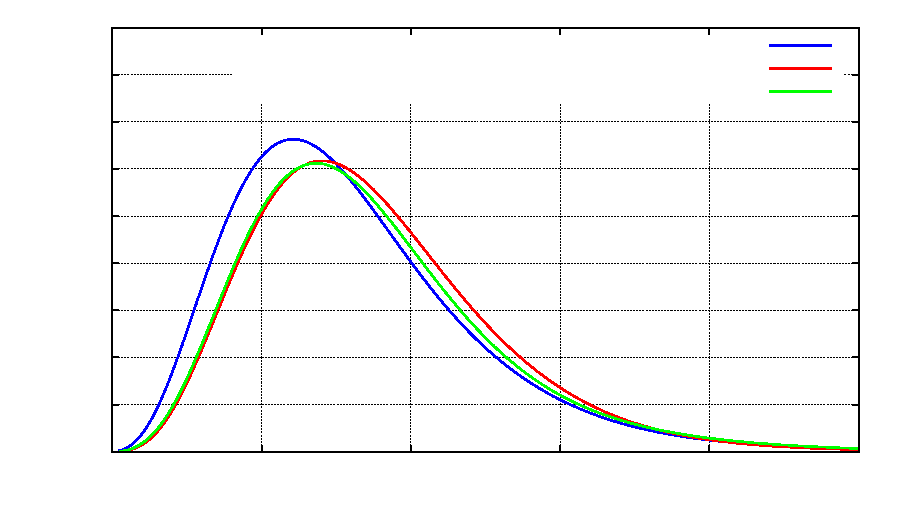
\includegraphics{graphs/elim}}%
    \gplfronttext
  \end{picture}%
\endgroup
}
  \caption{Histogram of $\log_{10}$ of absolute values of errors for one elimination and multiple elimination solvers.}
  \label{graph:elim}
\end{figure}

\begin{table}[ht]
  \centering
  \begin{tabular}{|c||ccc|}
    \hline
      & \textbf{One elimination} & \textbf{Multiple elimination} & \textbf{Multiple elimination} \\
      & \textbf{solver}          & \textbf{solver} ($step = 1$)  & \textbf{solver} ($step = 2$)\\
    \hline\hline
    \textbf{minimal} & 1.988 & 1.036 & 1.745\\
\textbf{median} & 2.799 & 2.003 & 2.198\\
\textbf{maximal} & 2.859 & 2.227 & 2.283\\

    \hline
  \end{tabular}
  \caption{Computing times of one and multiple elimination solvers.}
  \label{tab:elim}
\end{table}

You can see that the numerical stability of the multiple elimination solvers is slightly worse than the numerical stability of the one elimination solver. In the contrary, the multi elimination solvers are approximately 1.5 times faster than the one elimination solver. Interesting is that the second and third solvers are equivalently fast, but one of them consists of four eliminations and the second one only of two eliminations. Therefore, we can not say that more eliminations lead to faster solvers. So, it is important to run the benchmark to find the optimal number of eliminations for each minimal problem and then choose the best solver for the application.

\section{Matrix partitioning}
In this section, we compare the solvers using matrix partitioning as described in the section \ref{subsec:matrixPart}. For comparing, we have used multiple elimination solvers as described in the section \ref{subsec:multipleSolver}. We have set the variable $step$ to one so the generated solvers have four eliminations. The first solver has been generated without matrix partitioning. In the second one, matrix partitioning was used only for the last elimination and the third solver has been generated with matrix partitioning for all four eliminations used.

The benchmark templates used for this comparison are specified in the function \textit{bench\_\-mat\-rix\-Partitioning} in the folder \texttt{benchmark} in the automatic generator. The variable $step$ was set to 1 and all other settings have remained default.

The computing times of these tree solvers are in the Table \ref{tab:part} and the numerical stability is shown as histogram of $\log_{10}$ of absolute values of errors in the Figure \ref{graph:part}.

\begin{figure}[ht]
  \centering
  \resizebox{0.95\textwidth}{!}{% GNUPLOT: LaTeX picture with Postscript
\begingroup
  \makeatletter
  \providecommand\color[2][]{%
    \GenericError{(gnuplot) \space\space\space\@spaces}{%
      Package color not loaded in conjunction with
      terminal option `colourtext'%
    }{See the gnuplot documentation for explanation.%
    }{Either use 'blacktext' in gnuplot or load the package
      color.sty in LaTeX.}%
    \renewcommand\color[2][]{}%
  }%
  \providecommand\includegraphics[2][]{%
    \GenericError{(gnuplot) \space\space\space\@spaces}{%
      Package graphicx or graphics not loaded%
    }{See the gnuplot documentation for explanation.%
    }{The gnuplot epslatex terminal needs graphicx.sty or graphics.sty.}%
    \renewcommand\includegraphics[2][]{}%
  }%
  \providecommand\rotatebox[2]{#2}%
  \@ifundefined{ifGPcolor}{%
    \newif\ifGPcolor
    \GPcolorfalse
  }{}%
  \@ifundefined{ifGPblacktext}{%
    \newif\ifGPblacktext
    \GPblacktexttrue
  }{}%
  % define a \g@addto@macro without @ in the name:
  \let\gplgaddtomacro\g@addto@macro
  % define empty templates for all commands taking text:
  \gdef\gplbacktext{}%
  \gdef\gplfronttext{}%
  \makeatother
  \ifGPblacktext
    % no textcolor at all
    \def\colorrgb#1{}%
    \def\colorgray#1{}%
  \else
    % gray or color?
    \ifGPcolor
      \def\colorrgb#1{\color[rgb]{#1}}%
      \def\colorgray#1{\color[gray]{#1}}%
      \expandafter\def\csname LTw\endcsname{\color{white}}%
      \expandafter\def\csname LTb\endcsname{\color{black}}%
      \expandafter\def\csname LTa\endcsname{\color{black}}%
      \expandafter\def\csname LT0\endcsname{\color[rgb]{1,0,0}}%
      \expandafter\def\csname LT1\endcsname{\color[rgb]{0,1,0}}%
      \expandafter\def\csname LT2\endcsname{\color[rgb]{0,0,1}}%
      \expandafter\def\csname LT3\endcsname{\color[rgb]{1,0,1}}%
      \expandafter\def\csname LT4\endcsname{\color[rgb]{0,1,1}}%
      \expandafter\def\csname LT5\endcsname{\color[rgb]{1,1,0}}%
      \expandafter\def\csname LT6\endcsname{\color[rgb]{0,0,0}}%
      \expandafter\def\csname LT7\endcsname{\color[rgb]{1,0.3,0}}%
      \expandafter\def\csname LT8\endcsname{\color[rgb]{0.5,0.5,0.5}}%
    \else
      % gray
      \def\colorrgb#1{\color{black}}%
      \def\colorgray#1{\color[gray]{#1}}%
      \expandafter\def\csname LTw\endcsname{\color{white}}%
      \expandafter\def\csname LTb\endcsname{\color{black}}%
      \expandafter\def\csname LTa\endcsname{\color{black}}%
      \expandafter\def\csname LT0\endcsname{\color{black}}%
      \expandafter\def\csname LT1\endcsname{\color{black}}%
      \expandafter\def\csname LT2\endcsname{\color{black}}%
      \expandafter\def\csname LT3\endcsname{\color{black}}%
      \expandafter\def\csname LT4\endcsname{\color{black}}%
      \expandafter\def\csname LT5\endcsname{\color{black}}%
      \expandafter\def\csname LT6\endcsname{\color{black}}%
      \expandafter\def\csname LT7\endcsname{\color{black}}%
      \expandafter\def\csname LT8\endcsname{\color{black}}%
    \fi
  \fi
  \setlength{\unitlength}{0.0500bp}%
  \begin{picture}(8640.00,5040.00)%
    \gplgaddtomacro\gplbacktext{%
      \csname LTb\endcsname%
      \put(946,704){\makebox(0,0)[r]{\strut{} 0}}%
      \csname LTb\endcsname%
      \put(946,1156){\makebox(0,0)[r]{\strut{} 50}}%
      \csname LTb\endcsname%
      \put(946,1609){\makebox(0,0)[r]{\strut{} 100}}%
      \csname LTb\endcsname%
      \put(946,2061){\makebox(0,0)[r]{\strut{} 150}}%
      \csname LTb\endcsname%
      \put(946,2513){\makebox(0,0)[r]{\strut{} 200}}%
      \csname LTb\endcsname%
      \put(946,2966){\makebox(0,0)[r]{\strut{} 250}}%
      \csname LTb\endcsname%
      \put(946,3418){\makebox(0,0)[r]{\strut{} 300}}%
      \csname LTb\endcsname%
      \put(946,3870){\makebox(0,0)[r]{\strut{} 350}}%
      \csname LTb\endcsname%
      \put(946,4323){\makebox(0,0)[r]{\strut{} 400}}%
      \csname LTb\endcsname%
      \put(946,4775){\makebox(0,0)[r]{\strut{} 450}}%
      \csname LTb\endcsname%
      \put(1078,484){\makebox(0,0){\strut{}-15}}%
      \csname LTb\endcsname%
      \put(2511,484){\makebox(0,0){\strut{}-10}}%
      \csname LTb\endcsname%
      \put(3944,484){\makebox(0,0){\strut{}-5}}%
      \csname LTb\endcsname%
      \put(5377,484){\makebox(0,0){\strut{} 0}}%
      \csname LTb\endcsname%
      \put(6810,484){\makebox(0,0){\strut{} 5}}%
      \csname LTb\endcsname%
      \put(8243,484){\makebox(0,0){\strut{} 10}}%
      \put(176,2739){\rotatebox{-270}{\makebox(0,0){\strut{}Frequency}}}%
      \put(4660,154){\makebox(0,0){\strut{}log$_{10}\Big(\big|$error$\big|\Big)$}}%
      \put(4660,4665){\makebox(0,0){\strut{}}}%
    }%
    \gplgaddtomacro\gplfronttext{%
      \csname LTb\endcsname%
      \put(7256,4602){\makebox(0,0)[r]{\strut{}Without matrix partitioning}}%
      \csname LTb\endcsname%
      \put(7256,4382){\makebox(0,0)[r]{\strut{}Last elimination with matrix partitioning}}%
      \csname LTb\endcsname%
      \put(7256,4162){\makebox(0,0)[r]{\strut{}All eliminations with matrix partitioning}}%
    }%
    \gplbacktext
    \put(0,0){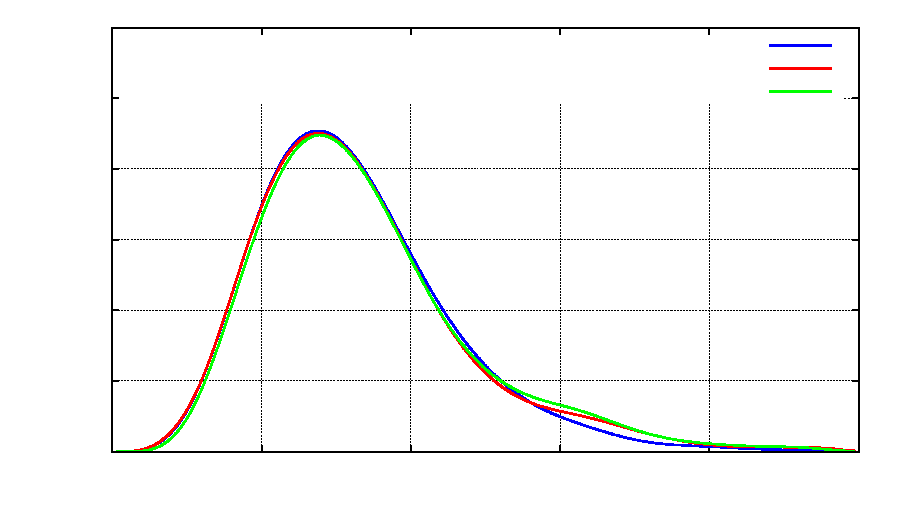
\includegraphics{graphs/part}}%
    \gplfronttext
  \end{picture}%
\endgroup
}
  \caption{Histogram of $\log_{10}$ of absolute values of errors for solver without matrix partitioning, solver with matrix partitioning only for the last elimination and solver with matrix partitioning for all eliminations in the solver.}
  \label{graph:part}
\end{figure}

\begin{table}[ht]
  \centering
  \begin{tabular}{|c||ccc|}
    \hline
      & \textbf{Without matrix} & \textbf{Matrix partitioning}      & \textbf{Matrix paritioning} \\
      & \textbf{partitioning}   & \textbf{for the last elimination} & \textbf{for all eliminations} \\
    \hline\hline
    \textbf{minimal time} & 1.353 s & 0.956 s & 0.794 s\\
\textbf{median of times} & 2.185 s & 1.071 s & 0.932 s\\
\textbf{maximal time} & 2.604 s & 1.189 s & 2.273 s\\

    \hline
  \end{tabular}
  \caption{Computing times of solver without matrix partitioning, of solver with matrix partitioning used for the last elimination and of solver with matrix partitioning used for all eliminations in the solver.}
  \label{tab:part}
\end{table}

We can see that the numerical stability remained the same for all three solvers. The solver with matrix partitioning for the last elimination used is approximately twice faster than solver without matrix paritioning. There is no big difference between the solver with matrix partitioning for the last elimination used and the solver with matrix partitioning used for all eliminations in the solver. The reason is, that when eliminating not the last matrix in the solver, we have to eliminate all the coupling columns. We do not have to do this when it is the last elimination. Therefore, the speed up of elimination of not the last matrix is not so big as the speed up of the last elimination.

\section{$F_4$ strategy}
At last, we have compared the solver generated by the systematical polynomial generator with solver generated with using the $F_4$ strategy. The first solver has been generated according to the decription in the section \ref{subsec:polynomialGenerator} using the systematical polynomial generator. The second one uses the $F_4$ strategy described in the section \ref{subsec:F4}.

We have used the benchmark templates that are defined in the function \textit{bench\_poly\-nomialGenerator} which is stored in the folder \texttt{benchmark} in the automatic generator. All other settings have remained default.

The numerical stability of both solvers are shown in the Figure \ref{graph:gen} as histogram of $\log_{10}$ of absolute values of errors. The computing times are in the Table \ref{tab:gen}.

\begin{figure}[ht]
  \centering
  \resizebox{0.95\textwidth}{!}{% GNUPLOT: LaTeX picture with Postscript
\begingroup
  \makeatletter
  \providecommand\color[2][]{%
    \GenericError{(gnuplot) \space\space\space\@spaces}{%
      Package color not loaded in conjunction with
      terminal option `colourtext'%
    }{See the gnuplot documentation for explanation.%
    }{Either use 'blacktext' in gnuplot or load the package
      color.sty in LaTeX.}%
    \renewcommand\color[2][]{}%
  }%
  \providecommand\includegraphics[2][]{%
    \GenericError{(gnuplot) \space\space\space\@spaces}{%
      Package graphicx or graphics not loaded%
    }{See the gnuplot documentation for explanation.%
    }{The gnuplot epslatex terminal needs graphicx.sty or graphics.sty.}%
    \renewcommand\includegraphics[2][]{}%
  }%
  \providecommand\rotatebox[2]{#2}%
  \@ifundefined{ifGPcolor}{%
    \newif\ifGPcolor
    \GPcolorfalse
  }{}%
  \@ifundefined{ifGPblacktext}{%
    \newif\ifGPblacktext
    \GPblacktexttrue
  }{}%
  % define a \g@addto@macro without @ in the name:
  \let\gplgaddtomacro\g@addto@macro
  % define empty templates for all commands taking text:
  \gdef\gplbacktext{}%
  \gdef\gplfronttext{}%
  \makeatother
  \ifGPblacktext
    % no textcolor at all
    \def\colorrgb#1{}%
    \def\colorgray#1{}%
  \else
    % gray or color?
    \ifGPcolor
      \def\colorrgb#1{\color[rgb]{#1}}%
      \def\colorgray#1{\color[gray]{#1}}%
      \expandafter\def\csname LTw\endcsname{\color{white}}%
      \expandafter\def\csname LTb\endcsname{\color{black}}%
      \expandafter\def\csname LTa\endcsname{\color{black}}%
      \expandafter\def\csname LT0\endcsname{\color[rgb]{1,0,0}}%
      \expandafter\def\csname LT1\endcsname{\color[rgb]{0,1,0}}%
      \expandafter\def\csname LT2\endcsname{\color[rgb]{0,0,1}}%
      \expandafter\def\csname LT3\endcsname{\color[rgb]{1,0,1}}%
      \expandafter\def\csname LT4\endcsname{\color[rgb]{0,1,1}}%
      \expandafter\def\csname LT5\endcsname{\color[rgb]{1,1,0}}%
      \expandafter\def\csname LT6\endcsname{\color[rgb]{0,0,0}}%
      \expandafter\def\csname LT7\endcsname{\color[rgb]{1,0.3,0}}%
      \expandafter\def\csname LT8\endcsname{\color[rgb]{0.5,0.5,0.5}}%
    \else
      % gray
      \def\colorrgb#1{\color{black}}%
      \def\colorgray#1{\color[gray]{#1}}%
      \expandafter\def\csname LTw\endcsname{\color{white}}%
      \expandafter\def\csname LTb\endcsname{\color{black}}%
      \expandafter\def\csname LTa\endcsname{\color{black}}%
      \expandafter\def\csname LT0\endcsname{\color{black}}%
      \expandafter\def\csname LT1\endcsname{\color{black}}%
      \expandafter\def\csname LT2\endcsname{\color{black}}%
      \expandafter\def\csname LT3\endcsname{\color{black}}%
      \expandafter\def\csname LT4\endcsname{\color{black}}%
      \expandafter\def\csname LT5\endcsname{\color{black}}%
      \expandafter\def\csname LT6\endcsname{\color{black}}%
      \expandafter\def\csname LT7\endcsname{\color{black}}%
      \expandafter\def\csname LT8\endcsname{\color{black}}%
    \fi
  \fi
  \setlength{\unitlength}{0.0500bp}%
  \begin{picture}(8640.00,5040.00)%
    \gplgaddtomacro\gplbacktext{%
      \csname LTb\endcsname%
      \put(946,704){\makebox(0,0)[r]{\strut{} 0}}%
      \csname LTb\endcsname%
      \put(946,1156){\makebox(0,0)[r]{\strut{} 100}}%
      \csname LTb\endcsname%
      \put(946,1609){\makebox(0,0)[r]{\strut{} 200}}%
      \csname LTb\endcsname%
      \put(946,2061){\makebox(0,0)[r]{\strut{} 300}}%
      \csname LTb\endcsname%
      \put(946,2513){\makebox(0,0)[r]{\strut{} 400}}%
      \csname LTb\endcsname%
      \put(946,2966){\makebox(0,0)[r]{\strut{} 500}}%
      \csname LTb\endcsname%
      \put(946,3418){\makebox(0,0)[r]{\strut{} 600}}%
      \csname LTb\endcsname%
      \put(946,3870){\makebox(0,0)[r]{\strut{} 700}}%
      \csname LTb\endcsname%
      \put(946,4323){\makebox(0,0)[r]{\strut{} 800}}%
      \csname LTb\endcsname%
      \put(946,4775){\makebox(0,0)[r]{\strut{} 900}}%
      \csname LTb\endcsname%
      \put(1078,484){\makebox(0,0){\strut{}-15}}%
      \csname LTb\endcsname%
      \put(2272,484){\makebox(0,0){\strut{}-10}}%
      \csname LTb\endcsname%
      \put(3466,484){\makebox(0,0){\strut{}-5}}%
      \csname LTb\endcsname%
      \put(4661,484){\makebox(0,0){\strut{} 0}}%
      \csname LTb\endcsname%
      \put(5855,484){\makebox(0,0){\strut{} 5}}%
      \csname LTb\endcsname%
      \put(7049,484){\makebox(0,0){\strut{} 10}}%
      \csname LTb\endcsname%
      \put(8243,484){\makebox(0,0){\strut{} 15}}%
      \put(176,2739){\rotatebox{-270}{\makebox(0,0){\strut{}Frequency}}}%
      \put(4660,154){\makebox(0,0){\strut{}log$_{10}$($|$error$|$)}}%
      \put(4660,4665){\makebox(0,0){\strut{}}}%
    }%
    \gplgaddtomacro\gplfronttext{%
      \csname LTb\endcsname%
      \put(7256,4602){\makebox(0,0)[r]{\strut{}Without matrix partitioning}}%
      \csname LTb\endcsname%
      \put(7256,4382){\makebox(0,0)[r]{\strut{}Last elimination with matrix partitioning}}%
    }%
    \gplbacktext
    \put(0,0){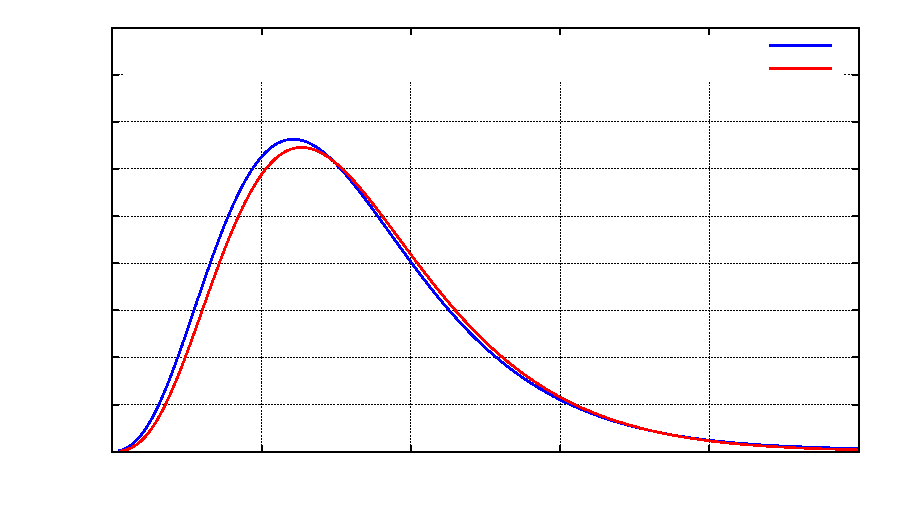
\includegraphics{graphs/gen}}%
    \gplfronttext
  \end{picture}%
\endgroup
}
  \caption{Histogram of $\log_{10}$ of absolute values of errors for solver generated by the systematical generator and for solver using the $F_4$ strategy.}
  \label{graph:gen}
\end{figure}

\begin{table}[ht]
  \centering
  \begin{tabular}{|c||cc|}
    \hline
    & \textbf{Systematical}    & \textbf{$F_4$ strategy} \\
    &  \textbf{generator used} & \textbf{used} \\
    \hline\hline
    \textbf{minimal} & 2.213 & 0.615\\
\textbf{median} & 2.895 & 0.713\\
\textbf{maximal} & 3.320 & 1.161\\

    \hline
  \end{tabular}
  \caption{Computing times of solver generated by the systematical generator and of the solver using the $F_4$ strategy.}
  \label{tab:gen}
\end{table}

From the results, we can see that the numerical stability has remained the same for both solvers. The solver which uses the $F_4$ strategy is about 4 times faster that the solver generated by the systematical polynomial generator.


\chapter{Conclusion}
In this work, we have focused on how to solve systems of polynomial equations fast and how to automatically generate efficient solvers for these systems.

In the first part, we have reviewed the state of the art algorithms for computing Gr\"obner basis of polynomial systems. We have described the Buchberger Algorithm \cite{Buchberger65}, then we have explained the $F_4$ Algorithm \cite{F4} in details and in the end, we have pointed out the main features of the $F_5$ Algorithm \cite{F5}.

In the second part, the automatic generator \cite{AutoGen} of minimal problem solvers has been presented. This tool enables us to easily generate solvers for systems of polynomial equations which arise when solving minimal problems in computer vision. We have described the process of generation of solvers in details. Then, we have suggested some improvements of the automatic generator and we have implemented them. For example, we have presented an improvement which allows us to generate multiple elimination solvers which are usually better for systems of polynomial equations in many unknowns. We have also shown that the solvers can be sped up when Gauss-Jordan elimination for sparse matrices is used. Next, we have taken over a strategy from the $F_4$ Algorithm \cite{F4} and we have implemented it into the automatic generator. For better understanding, we have implemented the $F_4$ Algorithm \cite{F4} in Maple first. The description of this implementation is provided in this section, too. In the end, we have presented the benchmark of the automatic generator. This tool helps us to decide which generated solver is better for our application.

In the end, we have taken the 9-point relative pose different radial distortion problem \cite{9pt} and compared solvers generated with different methods for this problem on set of randomly generated data. We have shown that solvers generated with the new implemented methods may be faster than solvers generated by the old implementation of the automatic generator. We have register the most visible speed up when the $F_4$ strategy is used. In this case, the solver using the $F_4$ strategy is four times faster than the solver generated by the systematical generator for the 9-point relative pose problem \cite{9pt}.


%\appendix
%\include{app01}

\bibliographystyle{plain}
\bibliography{citations}{}

\end{document}
